% Options for packages loaded elsewhere
\PassOptionsToPackage{unicode}{hyperref}
\PassOptionsToPackage{hyphens}{url}
%
\documentclass[
  english,
  man]{apa6}
\usepackage{lmodern}
\usepackage{amsmath}
\usepackage{ifxetex,ifluatex}
\ifnum 0\ifxetex 1\fi\ifluatex 1\fi=0 % if pdftex
  \usepackage[T1]{fontenc}
  \usepackage[utf8]{inputenc}
  \usepackage{textcomp} % provide euro and other symbols
  \usepackage{amssymb}
\else % if luatex or xetex
  \usepackage{unicode-math}
  \defaultfontfeatures{Scale=MatchLowercase}
  \defaultfontfeatures[\rmfamily]{Ligatures=TeX,Scale=1}
\fi
% Use upquote if available, for straight quotes in verbatim environments
\IfFileExists{upquote.sty}{\usepackage{upquote}}{}
\IfFileExists{microtype.sty}{% use microtype if available
  \usepackage[]{microtype}
  \UseMicrotypeSet[protrusion]{basicmath} % disable protrusion for tt fonts
}{}
\makeatletter
\@ifundefined{KOMAClassName}{% if non-KOMA class
  \IfFileExists{parskip.sty}{%
    \usepackage{parskip}
  }{% else
    \setlength{\parindent}{0pt}
    \setlength{\parskip}{6pt plus 2pt minus 1pt}}
}{% if KOMA class
  \KOMAoptions{parskip=half}}
\makeatother
\usepackage{xcolor}
\IfFileExists{xurl.sty}{\usepackage{xurl}}{} % add URL line breaks if available
\IfFileExists{bookmark.sty}{\usepackage{bookmark}}{\usepackage{hyperref}}
\hypersetup{
  pdftitle={Relationship between social capital and election results},
  pdfauthor={Anisha Babu1, Hyeonjin Cha1, Diana DeWald1, \& Murat Kezer1},
  pdflang={en-EN},
  pdfkeywords={keywords},
  hidelinks,
  pdfcreator={LaTeX via pandoc}}
\urlstyle{same} % disable monospaced font for URLs
\usepackage{graphicx}
\makeatletter
\def\maxwidth{\ifdim\Gin@nat@width>\linewidth\linewidth\else\Gin@nat@width\fi}
\def\maxheight{\ifdim\Gin@nat@height>\textheight\textheight\else\Gin@nat@height\fi}
\makeatother
% Scale images if necessary, so that they will not overflow the page
% margins by default, and it is still possible to overwrite the defaults
% using explicit options in \includegraphics[width, height, ...]{}
\setkeys{Gin}{width=\maxwidth,height=\maxheight,keepaspectratio}
% Set default figure placement to htbp
\makeatletter
\def\fps@figure{htbp}
\makeatother
\setlength{\emergencystretch}{3em} % prevent overfull lines
\providecommand{\tightlist}{%
  \setlength{\itemsep}{0pt}\setlength{\parskip}{0pt}}
\setcounter{secnumdepth}{-\maxdimen} % remove section numbering
% Make \paragraph and \subparagraph free-standing
\ifx\paragraph\undefined\else
  \let\oldparagraph\paragraph
  \renewcommand{\paragraph}[1]{\oldparagraph{#1}\mbox{}}
\fi
\ifx\subparagraph\undefined\else
  \let\oldsubparagraph\subparagraph
  \renewcommand{\subparagraph}[1]{\oldsubparagraph{#1}\mbox{}}
\fi
% Manuscript styling
\usepackage{upgreek}
\captionsetup{font=singlespacing,justification=justified}

% Table formatting
\usepackage{longtable}
\usepackage{lscape}
% \usepackage[counterclockwise]{rotating}   % Landscape page setup for large tables
\usepackage{multirow}		% Table styling
\usepackage{tabularx}		% Control Column width
\usepackage[flushleft]{threeparttable}	% Allows for three part tables with a specified notes section
\usepackage{threeparttablex}            % Lets threeparttable work with longtable

% Create new environments so endfloat can handle them
% \newenvironment{ltable}
%   {\begin{landscape}\begin{center}\begin{threeparttable}}
%   {\end{threeparttable}\end{center}\end{landscape}}
\newenvironment{lltable}{\begin{landscape}\begin{center}\begin{ThreePartTable}}{\end{ThreePartTable}\end{center}\end{landscape}}

% Enables adjusting longtable caption width to table width
% Solution found at http://golatex.de/longtable-mit-caption-so-breit-wie-die-tabelle-t15767.html
\makeatletter
\newcommand\LastLTentrywidth{1em}
\newlength\longtablewidth
\setlength{\longtablewidth}{1in}
\newcommand{\getlongtablewidth}{\begingroup \ifcsname LT@\roman{LT@tables}\endcsname \global\longtablewidth=0pt \renewcommand{\LT@entry}[2]{\global\advance\longtablewidth by ##2\relax\gdef\LastLTentrywidth{##2}}\@nameuse{LT@\roman{LT@tables}} \fi \endgroup}

% \setlength{\parindent}{0.5in}
% \setlength{\parskip}{0pt plus 0pt minus 0pt}

% \usepackage{etoolbox}
\makeatletter
\patchcmd{\HyOrg@maketitle}
  {\section{\normalfont\normalsize\abstractname}}
  {\section*{\normalfont\normalsize\abstractname}}
  {}{\typeout{Failed to patch abstract.}}
\patchcmd{\HyOrg@maketitle}
  {\section{\protect\normalfont{\@title}}}
  {\section*{\protect\normalfont{\@title}}}
  {}{\typeout{Failed to patch title.}}
\makeatother
\shorttitle{Title}
\keywords{keywords\newline\indent Word count: X}
\DeclareDelayedFloatFlavor{ThreePartTable}{table}
\DeclareDelayedFloatFlavor{lltable}{table}
\DeclareDelayedFloatFlavor*{longtable}{table}
\makeatletter
\renewcommand{\efloat@iwrite}[1]{\immediate\expandafter\protected@write\csname efloat@post#1\endcsname{}}
\makeatother
\usepackage{csquotes}
\ifxetex
  % Load polyglossia as late as possible: uses bidi with RTL langages (e.g. Hebrew, Arabic)
  \usepackage{polyglossia}
  \setmainlanguage[]{english}
\else
  \usepackage[shorthands=off,main=english]{babel}
\fi
\ifluatex
  \usepackage{selnolig}  % disable illegal ligatures
\fi
\usepackage[]{biblatex}
\addbibresource{r-references.bib}
\newlength{\cslhangindent}
\setlength{\cslhangindent}{1.5em}
\newlength{\csllabelwidth}
\setlength{\csllabelwidth}{3em}
\newenvironment{CSLReferences}[3] % #1 hanging-ident, #2 entry spacing
 {% don't indent paragraphs
  \setlength{\parindent}{0pt}
  % turn on hanging indent if param 1 is 1
  \ifodd #1 \everypar{\setlength{\hangindent}{\cslhangindent}}\ignorespaces\fi
  % set entry spacing
  \ifnum #2 > 0
  \setlength{\parskip}{#2\baselineskip}
  \fi
 }%
 {}
\usepackage{calc} % for \widthof, \maxof
\newcommand{\CSLBlock}[1]{#1\hfill\break}
\newcommand{\CSLLeftMargin}[1]{\parbox[t]{\maxof{\widthof{#1}}{\csllabelwidth}}{#1}}
\newcommand{\CSLRightInline}[1]{\parbox[t]{\linewidth}{#1}}
\newcommand{\CSLIndent}[1]{\hspace{\cslhangindent}#1}

\title{Relationship between social capital and election results}
\author{Anisha Babu\textsuperscript{1}, Hyeonjin Cha\textsuperscript{1}, Diana DeWald\textsuperscript{1}, \& Murat Kezer\textsuperscript{1}}
\date{}


\authornote{

Add complete departmental affiliations for each author here. Each new line herein must be indented, like this line.
Enter author note here.

The authors made the following contributions. Anisha Babu: Conceptualization, Data Analysis, Writing - Original Draft Preparation, Writing - Review \& Editing; Hyeonjin Cha: Conceptualization, Data Analysis, Writing - Original Draft Preparation, Writing - Review \& Editing; Diana DeWald: Conceptualization, Data Analysis, Writing - Original Draft Preparation, Writing - Review \& Editing; Murat Kezer: Conceptualization, Data Analysis, Writing - Original Draft Preparation, Writing - Review \& Editing.

}

\affiliation{\vspace{0.5cm}\textsuperscript{1} University of Oregon}

\abstract{
One or two sentences providing a \textbf{basic introduction} to the field, comprehensible to a scientist in any discipline.

Two to three sentences of \textbf{more detailed background}, comprehensible to scientists in related disciplines.

One sentence clearly stating the \textbf{general problem} being addressed by this particular study.

One sentence summarizing the main result (with the words ``\textbf{here we show}'' or their equivalent).

Two or three sentences explaining what the \textbf{main result} reveals in direct comparison to what was thought to be the case previously, or how the main result adds to previous knowledge.

One or two sentences to put the results into a more \textbf{general context}.

Two or three sentences to provide a \textbf{broader perspective}, readily comprehensible to a scientist in any discipline.
}



\begin{document}
\maketitle

\hypertarget{introduction}{%
\section{Introduction}\label{introduction}}

\hypertarget{methods}{%
\section{Methods}\label{methods}}

We report how we determined our sample size, all data exclusions (if any), all manipulations, and all measures in the study.

\hypertarget{data}{%
\subsection{Data}\label{data}}

The present study uses secondary datasets. First, \emph{The production of social capital in US counties constitutes the social capital data} (Rupasingha, Goetz, \& Freshwater, 2006, with updates){[}link{]}. Second, \emph{County Presidential Election Returns 2000-2016} (MIT Election Data and Science Lab, 2018) is used for presidential election results. Both datasets provide data on county level.

\hypertarget{data-preparation}{%
\subsection{Data Preparation}\label{data-preparation}}

To prepare the data for analysis, we started with the election data as it is more comprehensive in terms of the number of counties. First, we selected the variables of interests. Then, we selected the election years (i.e., 2000, 2008, 2012, 2016) that match with social capital data. The name of the year variable was changed in a way that shows it is the year of election so that it is not mixed with the same year variable in social capital data. Next, we create new datasets for each presidential election we are interested in. These will be later merged with corresponding social capital data.\\
For each social capital dataset (i.e., 1997, 2005, 2009, 2014), we first added state code for some counties that do not readily contain that information. Then, we created two variables out of the area name such that we have different variables for county names and state codes. Then, we selected the relevant variables and cleaned the variable names. We only selected the variables that were available for all time points that we chose. Next, we created a year variable indicating when the data were collected.\\
Finally, we reorder the variables so that they are the same across datasets, and merged the four datasets to create one dataset that contains all of the data from each dataset.

\hypertarget{data-analysis}{%
\subsection{Data analysis}\label{data-analysis}}

<<<<<<< HEAD
<<<<<<< Updated upstream
We used R \autocite[Version 3.6.1;][]{R-base} and the R-packages \emph{dplyr} \autocite[Version 1.0.0;][]{R-dplyr}, \emph{forcats} \autocite[Version 0.5.0;][]{R-forcats}, \emph{ggplot2} \autocite[Version 3.3.2;][]{R-ggplot2}, \emph{here} \autocite[Version 0.1;][]{R-here}, \emph{janitor} \autocite[Version 2.0.1;][]{R-janitor}, \emph{kableExtra} \autocite[Version 1.3.1;][]{R-kableExtra}, \emph{knitr} \autocite[Version 1.29;][]{R-knitr}, \emph{magrittr} \autocite[Version 1.5;][]{R-magrittr}, \emph{papaja} \autocite[Version 0.1.0.9997;][]{R-papaja}, \emph{purrr} \autocite[Version 0.3.4;][]{R-purrr}, \emph{readr} \autocite[Version 1.3.1;][]{R-readr}, \emph{rio} \autocite[Version 0.5.16;][]{R-rio}, \emph{stringr} \autocite[Version 1.4.0;][]{R-stringr}, \emph{tibble} \autocite[Version 3.0.2;][]{R-tibble}, \emph{tidyr} \autocite[Version 1.1.0;][]{R-tidyr}, and \emph{tidyverse} \autocite[Version 1.3.0;][]{R-tidyverse} for all our analyses.

\begin{verbatim}
## Warning: `...` is not empty.
## 
## We detected these problematic arguments:
## * `needs_dots`
## 
## These dots only exist to allow future extensions and should be empty.
## Did you misspecify an argument?

## Warning: `...` is not empty.
## 
## We detected these problematic arguments:
## * `needs_dots`
## 
## These dots only exist to allow future extensions and should be empty.
## Did you misspecify an argument?
\end{verbatim}
=======
We used R (Version 4.0.2; R Core Team, 2020) and the R-packages \emph{dplyr} (Version 1.0.2; Wickham et al., 2020), \emph{forcats} (Version 0.5.0; Wickham, 2020a), \emph{ggplot2} (Version 3.3.2; Wickham, 2016), \emph{here} (Version 0.1; Müller, 2017), \emph{janitor} (Version 2.0.1; Firke, 2020), \emph{kableExtra} (Version 1.3.1; Zhu, 2020), \emph{knitr} (Version 1.30; Xie, 2015), \emph{magrittr} (Version 1.5; Bache \& Wickham, 2014), \emph{papaja} (Version 0.1.0.9997; Aust \& Barth, 2020), \emph{purrr} (Version 0.3.4; Henry \& Wickham, 2020), \emph{readr} (Version 1.3.1; Wickham, Hester, \& Francois, 2018), \emph{rio} (Version 0.5.16; Chan, Chan, Leeper, \& Becker, 2018), \emph{stringr} (Version 1.4.0; Wickham, 2019), \emph{tibble} (Version 3.0.3; Müller \& Wickham, 2020), \emph{tidyr} (Version 1.1.2; Wickham, 2020b), and \emph{tidyverse} (Version 1.3.0; Wickham, Averick, et al., 2019) for all our analyses.
>>>>>>> Stashed changes
=======
First, we provide the descriptive statistics in Table 1-X. Next, we visualize the data. Finally, we present regression models in which elections results are predicted by different types of social capital.
We used R \autocite[Version 3.6.1;][]{R-base} and the R-packages \emph{broom} \autocite[Version 0.7.0;][]{R-broom}, \emph{corx} \autocite[Version 1.0.6.1;][]{R-corx}, \emph{dplyr} \autocite[Version 1.0.2;][]{R-dplyr}, \emph{forcats} \autocite[Version 0.5.0;][]{R-forcats}, \emph{ggplot2} \autocite[Version 3.3.2;][]{R-ggplot2}, \emph{gtsummary} \autocite[Version 1.3.5;][]{R-gtsummary}, \emph{here} \autocite[Version 0.1;][]{R-here}, \emph{janitor} \autocite[Version 2.0.1;][]{R-janitor}, \emph{kableExtra} \autocite[Version 1.3.1;][]{R-kableExtra}, \emph{knitr} \autocite[Version 1.29;][]{R-knitr}, \emph{magrittr} \autocite[Version 1.5;][]{R-magrittr}, \emph{papaja} \autocite[Version 0.1.0.9997;][]{R-papaja}, \emph{purrr} \autocite[Version 0.3.4;][]{R-purrr}, \emph{readr} \autocite[Version 1.3.1;][]{R-readr}, \emph{rio} \autocite[Version 0.5.16;][]{R-rio}, \emph{scales} \autocite[Version 1.1.1;][]{R-scales}, \emph{sjlabelled} \autocite[Version 1.1.7;][]{R-sjlabelled}, \emph{sjmisc} \autocite[Version 2.8.5;][]{R-sjmisc}, \emph{stringr} \autocite[Version 1.4.0;][]{R-stringr}, \emph{tibble} \autocite[Version 3.0.4;][]{R-tibble}, \emph{tidyr} \autocite[Version 1.1.2;][]{R-tidyr}, \emph{tidyverse} \autocite[Version 1.3.0;][]{R-tidyverse}, and \emph{usmap} \autocite[Version 0.5.1;][]{R-usmap} for all our analyses.
>>>>>>> main

\begin{table}

\caption{(\#tab:descriptives table 1)A summary table for votes by candidate and year of election.}
\centering
\begin{tabular}[t]{c|c|c|c|c}
\hline
Year & Party & N & Mean Candidate Votes & SD Candidate Votes\\
\hline
2000 & Dem & 3107 & 16218 & 57150\\
\hline
2000 & Green & 3107 & -- & --\\
\hline
2000 & Rep & 3107 & 16049 & 38632\\
\hline
2000 & -- & 3107 & 339 & 954\\
\hline
2008 & Dem & 3108 & 22157 & 76972\\
\hline
2008 & Rep & 3108 & 19167 & 44840\\
\hline
2008 & -- & 3108 & 577 & 1848\\
\hline
2012 & Dem & 3108 & 20974 & 73998\\
\hline
2012 & Rep & 3108 & 19409 & 44596\\
\hline
2012 & -- & 3108 & 838 & 2952\\
\hline
2016 & Dem & 3115 & 21071 & 80496\\
\hline
2016 & Rep & 3115 & 20160 & 43157\\
\hline
2016 & -- & 3115 & 2449 & 7509\\
\hline
\multicolumn{5}{l}{\rule{0pt}{1em}\textit{Note: } N = total number of counties in the US reporting data.}\\
\end{tabular}
\end{table}

\begin{table}

\caption{\label{tab:regression}Table X. Correlation between social capital variables (2014) and democratic margin (2016)}
\centering
\begin{tabular}[t]{l|c|c|c|c|c|c|c|c|c|c|c}
\hline
  & 1 & 2 & 3 & 4 & 5 & 6 & 7 & 8 & 9 & 10 & 11\\
\hline
1. Bowling & - &  &  &  &  &  &  &  &  &  & \\
\hline
2. Civic & .16* & - &  &  &  &  &  &  &  &  & \\
\hline
3. Golf & .18* & .17* & - &  &  &  &  &  &  &  & \\
\hline
4. Religious & .18* & .25* & .35* & - &  &  &  &  &  &  & \\
\hline
5. Sport & -.01 & .00 & -.02 & .00 & - &  &  &  &  &  & \\
\hline
6. Political & -.03 & .00 & -.03 & .00 & .01 & - &  &  &  &  & \\
\hline
7. Professional & -.01 & .08* & -.04* & -.03 & .02 & .20* & - &  &  &  & \\
\hline
8. Business & .10* & .14* & .14* & .31* & -.02 & .09* & .16* & - &  &  & \\
\hline
9. Labor & .01 & .13* & -.03 & -.05* & .02 & .05* & .11* & -.02 & - &  & \\
\hline
10. NonProfit & .22* & .35* & .28* & .37* & .02 & .09* & .14* & .33* & .00 & - & \\
\hline
11. Social Capital Index & .29* & .46* & .43* & .68* & .03 & .09* & .13* & .44* & .03 & .85* & -\\
\hline
12. Democratic Margin & -.09* & -.04* & -.14* & -.33* & .02 & .09* & .19* & -.09* & .13* & -.07* & -.14*\\
\hline
\multicolumn{12}{l}{\rule{0pt}{1em}\textit{Note: } * p < .05; ** p < .01; *** p < .001}\\
\end{tabular}
\end{table}

\begin{table}

\caption{\label{tab:regression}Table X. Correlation between social capital variables (2009) and democratic margin (2012)}
\centering
\begin{tabular}[t]{l|c|c|c|c|c|c|c|c|c|c|c}
\hline
  & 1 & 2 & 3 & 4 & 5 & 6 & 7 & 8 & 9 & 10 & 11\\
\hline
1. Bowling & - &  &  &  &  &  &  &  &  &  & \\
\hline
2. Civic & .21* & - &  &  &  &  &  &  &  &  & \\
\hline
3. Golf & .23* & .18* & - &  &  &  &  &  &  &  & \\
\hline
4. Religious & .23* & .23* & .42* & - &  &  &  &  &  &  & \\
\hline
5. Sport & -.02 & -.01 & -.02 & .00 & - &  &  &  &  &  & \\
\hline
6. Political & .00 & .05* & -.04* & -.01 & .01 & - &  &  &  &  & \\
\hline
7. Professional & .06* & .05* & -.04* & -.01 & .01 & .24* & - &  &  &  & \\
\hline
8. Business & .12* & .21* & .17* & .26* & -.02 & .15* & .22* & - &  &  & \\
\hline
9. Labor & .04* & .13* & -.05* & -.03 & .01 & .06* & .11* & -.04* & - &  & \\
\hline
10. NonProfit & .29* & .38* & .33* & .41* & .01 & .09* & .16* & .33* & .01 & - & \\
\hline
11. Social Capital Index & .36* & .47* & .48* & .65* & .03 & .10* & .16* & .41* & .05* & .86* & -\\
\hline
12. Democratic Margin & -.05* & .02 & -.10* & -.27* & .02 & .06* & .12* & -.12* & .19* & -.05* & -.08*\\
\hline
\multicolumn{12}{l}{\rule{0pt}{1em}\textit{Note: } * p < .05; ** p < .01; *** p < .001}\\
\end{tabular}
\end{table}

\begin{table}

\caption{\label{tab:regression}Table X. Correlation between social capital variables (2005) and democratic margin (2008)}
\centering
\begin{tabular}[t]{l|c|c|c|c|c|c|c|c|c|c|c}
\hline
  & 1 & 2 & 3 & 4 & 5 & 6 & 7 & 8 & 9 & 10 & 11\\
\hline
1. Bowling & - &  &  &  &  &  &  &  &  &  & \\
\hline
2. Civic & .29* & - &  &  &  &  &  &  &  &  & \\
\hline
3. Golf & .23* & .18* & - &  &  &  &  &  &  &  & \\
\hline
4. Religious & .22* & .24* & .34* & - &  &  &  &  &  &  & \\
\hline
5. Sport & -.04* & .04* & -.05* & -.09* & - &  &  &  &  &  & \\
\hline
6. Political & -.02 & .04* & -.05* & -.01 & .05* & - &  &  &  &  & \\
\hline
7. Professional & .02 & .12* & -.03 & .03 & .12* & .21* & - &  &  &  & \\
\hline
8. Business & .11* & .13* & .16* & .26* & -.01 & .12* & .17* & - &  &  & \\
\hline
9. Labor & .02 & .15* & -.04* & -.01 & .14* & .12* & .10* & -.02 & - &  & \\
\hline
10. NonProfit & .30* & .37* & .29* & .40* & .02 & .06* & .18* & .30* & .02 & - & \\
\hline
11. Social Capital Index & .39* & .48* & .42* & .63* & .01 & .07* & .18* & .35* & .11* & .81* & -\\
\hline
12. Democratic Margin & -.04* & .08* & -.07* & -.23* & .14* & .06* & .12* & -.14* & .23* & -.03 & -.05*\\
\hline
\multicolumn{12}{l}{\rule{0pt}{1em}\textit{Note: } * p < .05; ** p < .01; *** p < .001}\\
\end{tabular}
\end{table}

\begin{table}

\caption{\label{tab:regression}Table X. Correlation between social capital variables (1997) and democratic margin (2000)}
\centering
\begin{tabular}[t]{l|c|c|c|c|c|c|c|c|c|c|c}
\hline
  & 1 & 2 & 3 & 4 & 5 & 6 & 7 & 8 & 9 & 10 & 11\\
\hline
1. Bowling & - &  &  &  &  &  &  &  &  &  & \\
\hline
2. Civic & .25* & - &  &  &  &  &  &  &  &  & \\
\hline
3. Golf & .22* & .18* & - &  &  &  &  &  &  &  & \\
\hline
4. Religious & .23* & .21* & .17* & - &  &  &  &  &  &  & \\
\hline
5. Sport & -.01 & .04* & .01 & .01 & - &  &  &  &  &  & \\
\hline
6. Political & -.02 & .05* & -.01 & -.06* & .04* & - &  &  &  &  & \\
\hline
7. Professional & .03 & .12* & -.03 & -.01 & .06* & .33* & - &  &  &  & \\
\hline
8. Business & .10* & .14* & .05* & .09* & .01 & .17* & .22* & - &  &  & \\
\hline
9. Labor & .03 & .14* & -.01 & -.04* & .03 & .10* & .08* & -.02 & - &  & \\
\hline
10. NonProfit & .39* & .44* & .24* & .39* & .04* & .06* & .18* & .30* & .00 & - & \\
\hline
11. Social Capital Index & .45* & .51* & .31* & .60* & .08* & .06* & .17* & .31* & .07* & .87* & -\\
\hline
12. Democratic Margin & -.15* & -.06* & -.13* & -.20* & .01 & .08* & .07* & -.08* & .25* & -.23* & -.26*\\
\hline
\multicolumn{12}{l}{\rule{0pt}{1em}\textit{Note: } * p < .05; ** p < .01; *** p < .001}\\
\end{tabular}
\end{table}

\begin{table}

\caption{\label{tab:regression}Table X. Social Capital Variables Regressed on Democratic Margin for Each Time Point}
\centering
\begin{tabular}[t]{c|c|c|c|c|c|c|c|c|c|c|c|c}
\hline
\multicolumn{1}{c|}{\textbf{ }} & \multicolumn{3}{c|}{\textbf{2000}} & \multicolumn{3}{c|}{\textbf{2004}} & \multicolumn{3}{c|}{\textbf{2008}} & \multicolumn{3}{c}{\textbf{2012}} \\
\cline{2-4} \cline{5-7} \cline{8-10} \cline{11-13}
Term & B & SE & p & B & SE & p & B & SE & p & B & SE & p\\
\hline
Intercept & -0.12 & 0.01 & <0.05 & -0.09 & 0.01 & <0.05 & -0.11 & 0.01 & <0.05 & -0.17 & 0.01 & <0.05\\
\hline
Religious & -0.09 & 0.01 & <0.05 & -0.15 & 0.01 & <0.05 & -0.16 & 0.01 & <0.05 & -0.21 & 0.01 & <0.05\\
\hline
Civic & -0.09 & 0.03 & <0.05 & 0.20 & 0.03 & <0.05 & 0.11 & 0.03 & <0.05 & 0.08 & 0.04 & 0.05\\
\hline
Labor & 0.89 & 0.06 & <0.05 & 1.03 & 0.08 & <0.05 & 0.90 & 0.09 & <0.05 & 0.65 & 0.10 & <0.05\\
\hline
\multicolumn{13}{l}{\rule{0pt}{1em}\textit{Note: } The headers indicate election years.}\\
\end{tabular}
\end{table}

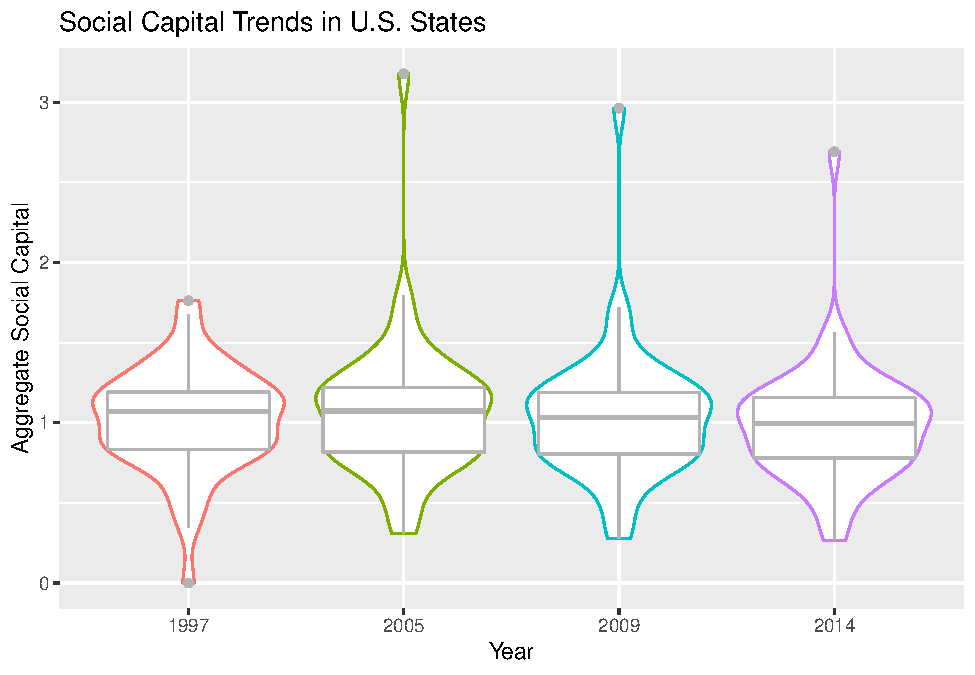
\includegraphics{Script_files/figure-latex/visualization part 1-1.pdf} 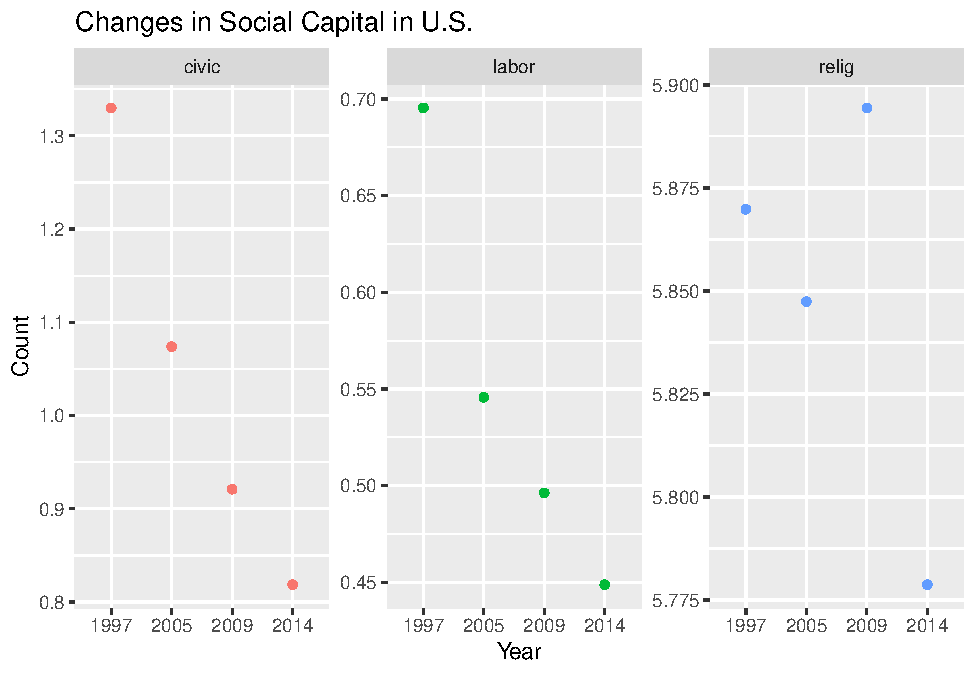
\includegraphics{Script_files/figure-latex/visualization part 1-2.pdf} 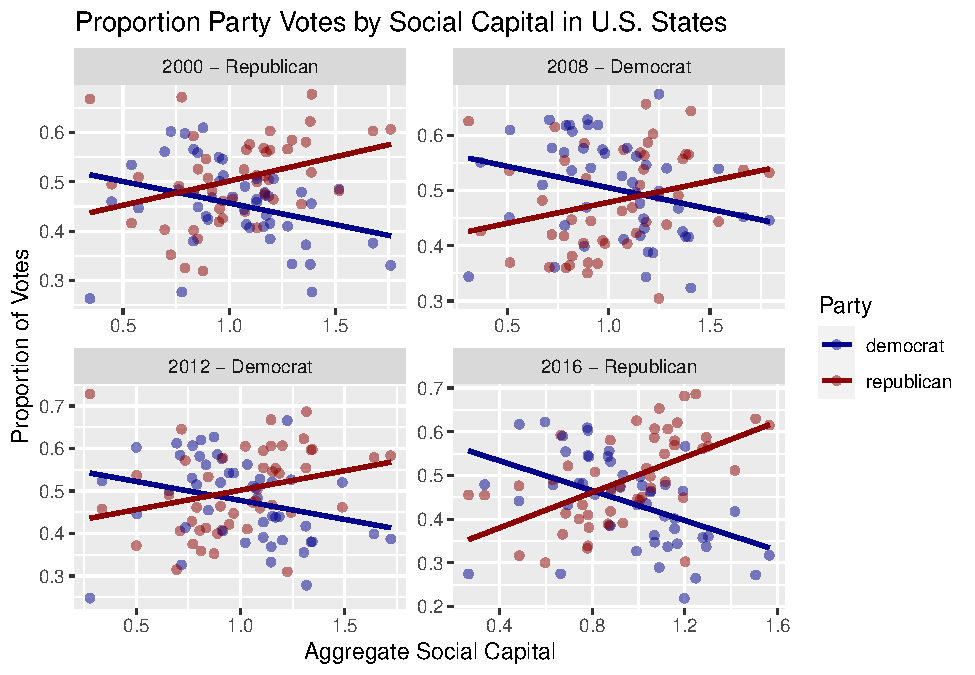
\includegraphics{Script_files/figure-latex/visualization part 1-3.pdf}

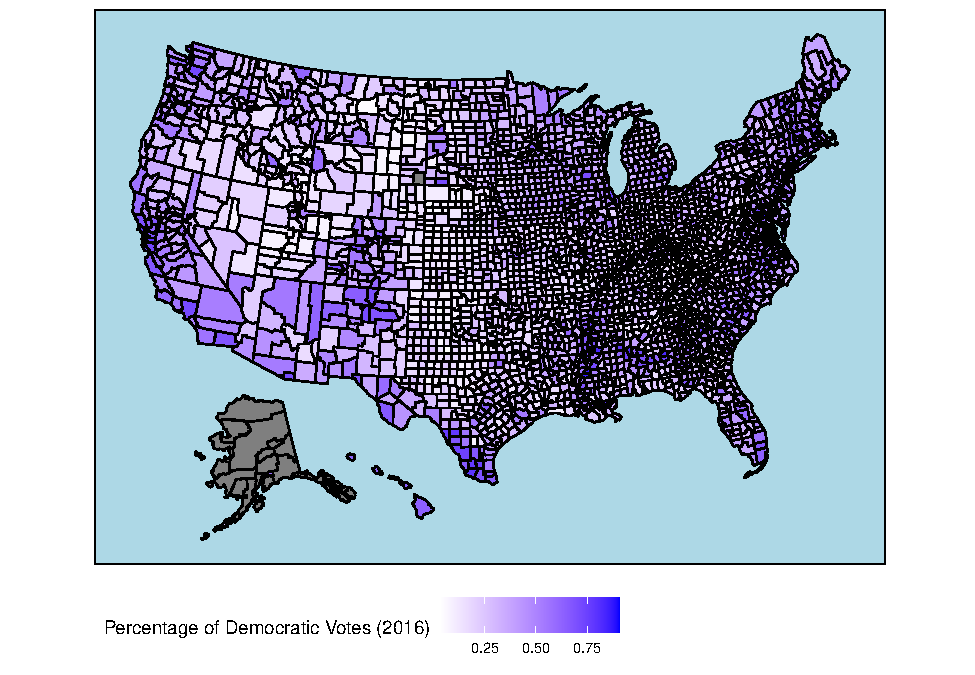
\includegraphics{Script_files/figure-latex/visualization part 2-1.pdf} 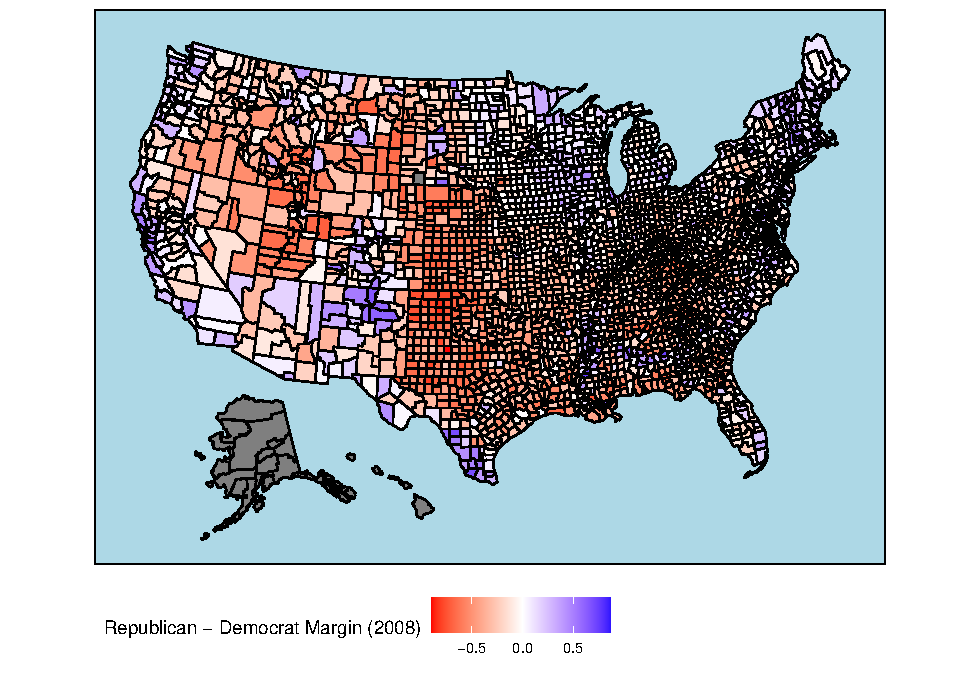
\includegraphics{Script_files/figure-latex/visualization part 2-2.pdf} 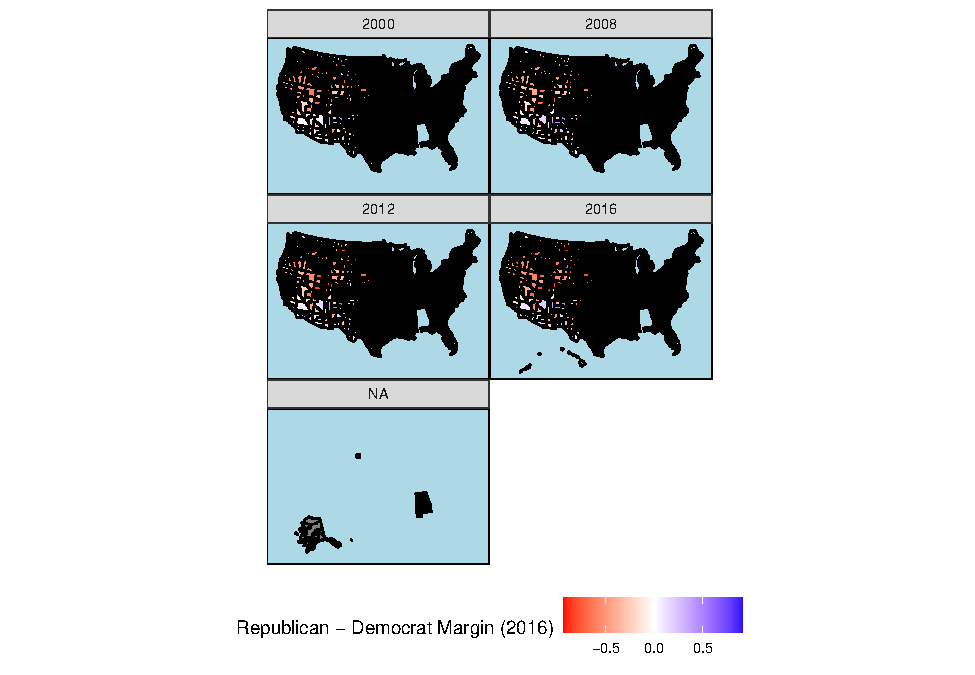
\includegraphics{Script_files/figure-latex/visualization part 2-3.pdf} 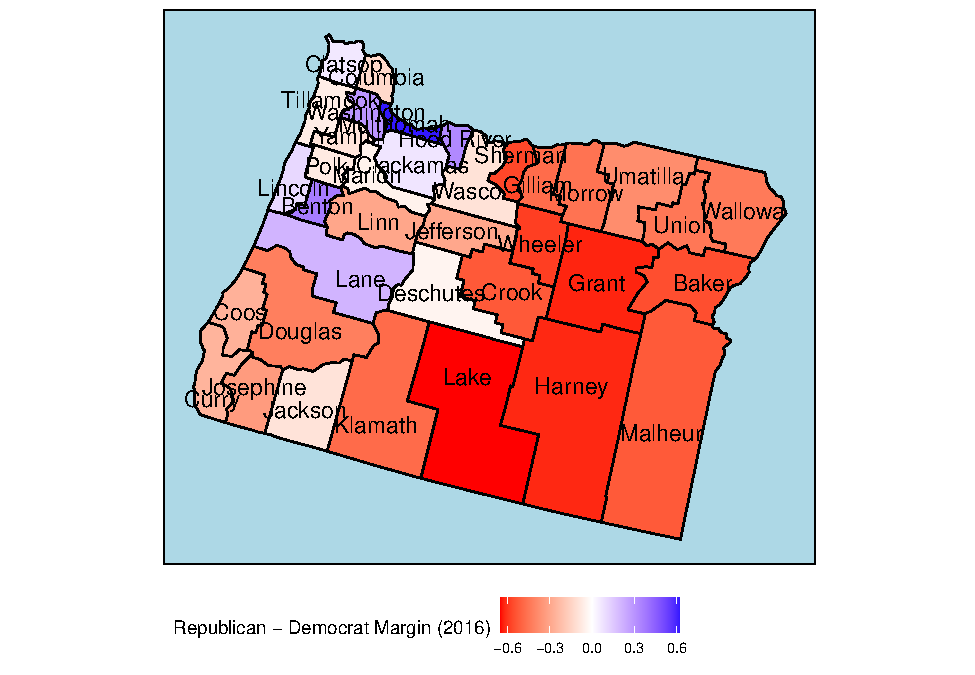
\includegraphics{Script_files/figure-latex/visualization part 2-4.pdf} 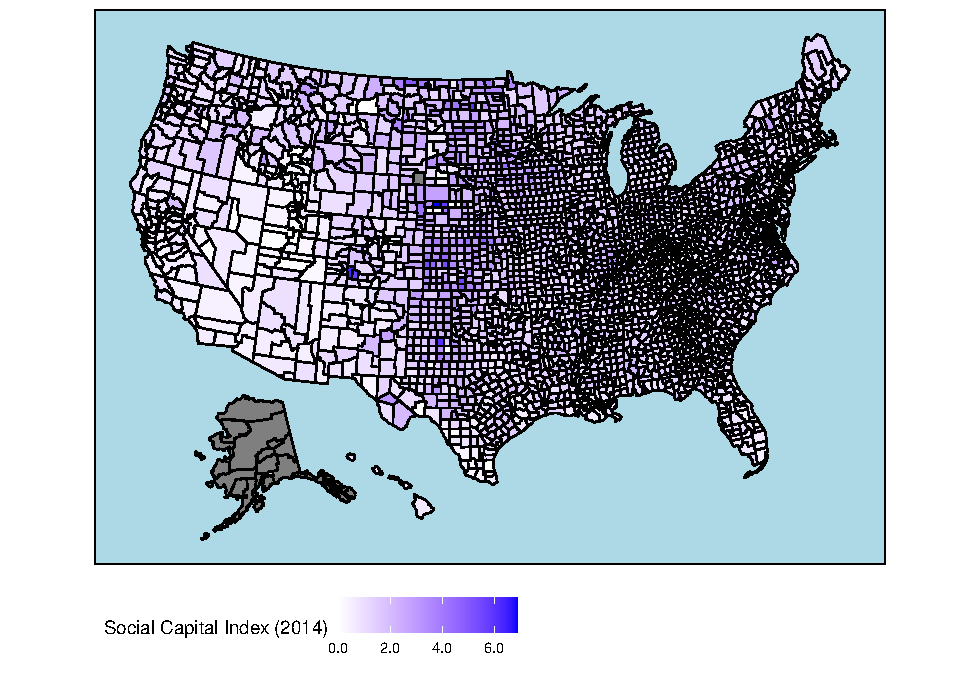
\includegraphics{Script_files/figure-latex/visualization part 2-5.pdf} 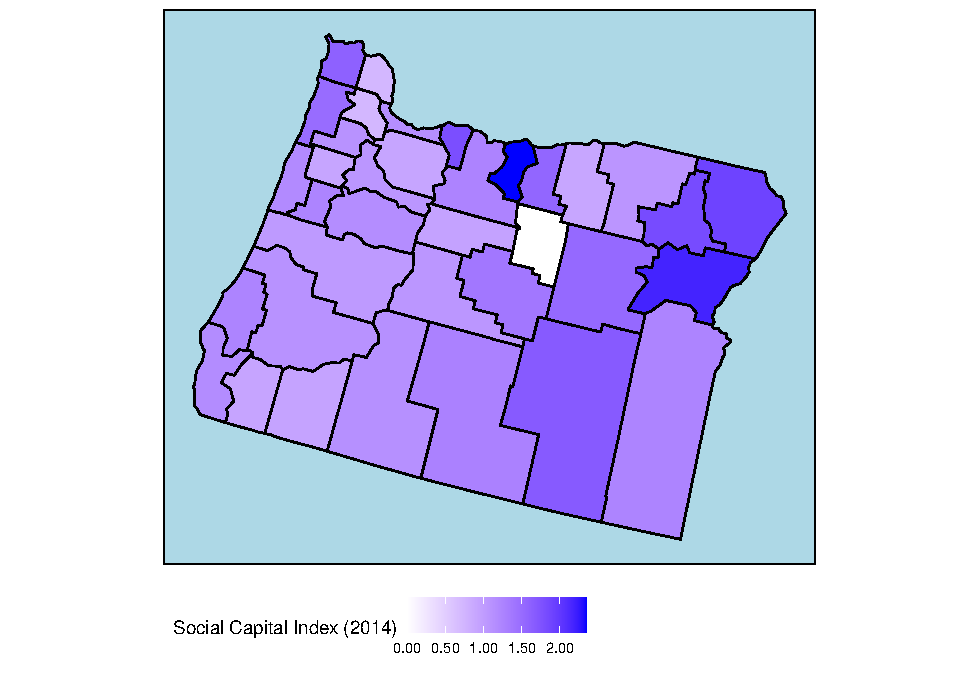
\includegraphics{Script_files/figure-latex/visualization part 2-6.pdf}

\hypertarget{results}{%
\section{Results}\label{results}}

\hypertarget{discussion}{%
\section{Discussion}\label{discussion}}

\newpage

\hypertarget{references}{%
\section{References}\label{references}}

\begingroup
\setlength{\parindent}{-0.5in}
\setlength{\leftskip}{0.5in}

\hypertarget{refs}{}
\begin{CSLReferences}{0}{0}
\end{CSLReferences}

\leavevmode\hypertarget{ref-R-kableExtra}{}%
Zhu, H. (2020). \emph{KableExtra: Construct complex table with 'kable' and pipe syntax}. Retrieved from \url{https://CRAN.R-project.org/package=kableExtra}

\endgroup


\printbibliography

\end{document}
